\documentclass[MasterThesisMain.tex]{subfiles}
\begin{document}
\chapter{Discussion}

\section{Experimental setup}
The experimental setup can be used in two ways. The first way with the optical fibre in the single point stage and the second way in the solvent vapour annealing chamber. When the optical fibre is fitted into the solvent vapour annealing chamber, the light must pass through a sapphire lens. This causes a great deal of reflected of light and effects the reflectance measurements taken. This can be seen by holding the static measurements seen in table \ref{tab:polymers} against the first fitted thickness values found in the figures for each polymer in chapter \ref{ch:results}. The effects may be small at the beginning of the solvent vapour annealing when the polymer has not swelled, but during swelling the reflectance measurement drops and can be zero in wavelength intervals. The sapphire lens effectively increases the dark measurement and when calculating the reflectance, since the dark measurement is in the denominator, lowers the reflectance measurements. If the thin film measurement decreases during the swelling this will also impact the reflectance measurement, lowering it even more. It can be seen when plotting the reflectance measurements alone with no strict axis interval that some reflectance measurements drops below zero, figure \ref{fig:drop}, the reason for this is unknown and close to zero ,figure \ref{fig:drop2}. The dark measurements are taken when the optical fibre is fitted into the solvent vapour annealing chamber with a piece of black fabric where the wafer would lay. The black fabric is a piece of black cotton which has been taken from a bit of clothing. The effect, if there is any, of the black fabric has not been investigated. The distance from the wafer to the optical fiber is important, as it is seen to shift the whole reflectance measurement up and down the y axis. Up if the distance increases and down if it decreases. It is therefore very important to use a step wafer where the thickness is known to adjust the single point stage before a static measurement of a wafer with a thin film. When the optical fiber is placed in the solvent vapour annealing chamber the distance between the optical fiber and the wafer is much greater than it intended thus the sapphire lens is used to focus the light to illuminate the wafer. Calibrating the solvent vapour annealing setup is impossible at this point since the chamber is not big enough for the step wafer to be place in the chamber. Taking the best reference and dark measurement is key to a good reflectance measurement for the thin film, though it seems that the best measurement is impossible, it seems that a measurement close to good can be achieved as seen in the fitting of the fresnel equations using the homopolymer reflectance data.

\begin{figure}[H]
\centering
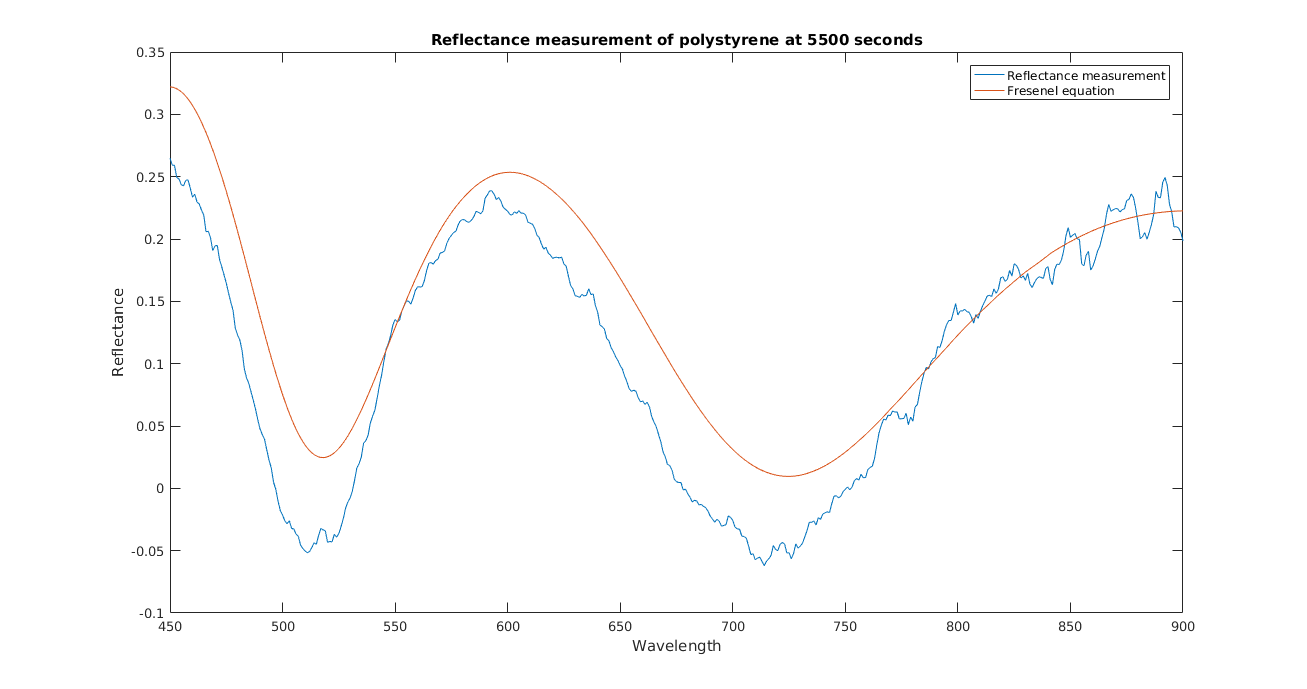
\includegraphics[width = \textwidth]{refldrop.png}
\caption{}
\label{fig:drop}
\end{figure}

\begin{figure}[H]
\centering
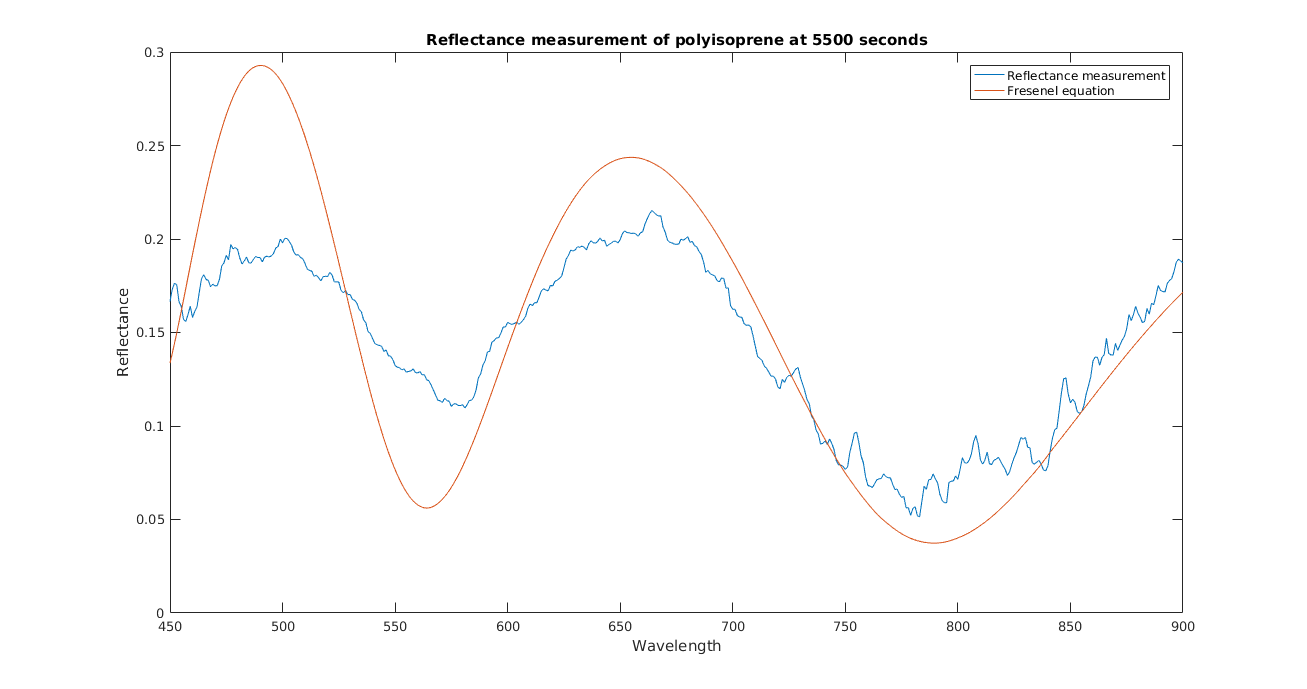
\includegraphics[width = \textwidth]{refldrop2.png}
\caption{}
\label{fig:drop2}
\end{figure}

\section{Refractive index dispersion of polymers and absorption}
The refractive index dispersion of the polymers has been shown in figure \ref{fig:dispshort} using the values given by the experimental method ellipsometry. It can be seen that the refractive index varies across the wavelengths. Polystyrene's refractive index does not vary as greatly as polyisoprene and the linear diblock copolymer polystyrene-b-polyisoprene. The fitting has not taken into account the dispersion of the refractive index, instead the constant refractive index has been used. It is unknown how the uptake of the solvent would effect the dispersion and how the dispersion would effect the reflectance measurements. An analytical study of the fresnel equations would be needed to fully grasp how changing the refractive indices impact the reflectance curves. Absorption is another parameter that can affect the reflectance measurements. Absorption is not present in the fresnel equations can can be the cause for the divergence between the reflectance measurements and the fresnel equations.    


\section{Mean square error fitting}
The mean square error fitting has been used as it was the fitting used in the nano-calc software and other fitting methods have not been studied or implemented.

\section{Solvent vapour annealing}

\section{Results}

\subsection{Polystyrene vs. Polyisoprene}

\subsection{Polystyrene/Polyisoprene vs. polystyrene-b-polyisoprene}

\end{document}